\documentclass[pageno]{jpaper}

%replace XXX with the submission number you are given from the HPCA submission site.
\newcommand{\hpcasubmissionnumber}{XXX}

\usepackage[normalem]{ulem}

\begin{document}

\title{Enhanced Base-Delta Compression with Data Splitting and Memory Pooling}
\author{Aditya Bhandaru (\href{mailto:akbhanda@andrew.cmu.edu}{akbhanda@andrew.cmu.edu}) Gennady Pekhimenko (\href{mailto:gpekhime@cs.cmu.edu}{akbhanda@andrew.cmu.edu}) \\
Onur Mutlu (\href{mailto:onur@cmu.edu}{akbhanda@andrew.cmu.edu})}
\date{}
\maketitle

\thispagestyle{empty}

\begin{abstract}
Recent literature on cache compression has shown great potential for increasing the effective cache capacity on chip. Specifically, a technique called Base-Delta (B+$\Delta$) compression has presented excellent compression (about 1.4X) and improvements in overall performance. However, B+$\Delta$ suffers from poor compressibility when adjacent data in memory have a high range in value.

We show here, as proof of concept, that existing techniques such as \textbf{Data Splitting and Memory Pooling can enhance B+$\Delta$ compressibility} for data in memory. Our simulations over various micro-benchmarks show that B+$\Delta$ with pooling  results in an 12\% increase in hit rate, and a compression ratio of 2.8X over the baseline.
\end{abstract}

\section{Introduction}

\subsection{Background}

The memory bottleneck is a well known problem in computer architecture. Caching has become a standard for alleviating contention for data, the bus, and memory. As we trend to more cores, more applications, and larger computing problems, there is a much greater demand for data. Simply scaling cache size to compensate is too expensive, both in power and chip area.

Data compression in the cache is a promising alternative to increasing effective on chip cache capacity. For the same physical cache space, we can store more blocks per set. In general, compression algorithms look for patterns in data to exploit. Therefore, they are very sensitive to how data is laid out in memory and the kind of data a program manipulates.

The ideal cache compression implementation would be fast, simple, and offer a high compression. These design points are largely at odds with one another. For example, many ideas from older literature on cache compression suffer from either poor compression or incur high hardware complexity or long decompression latencies.

Why is fast decompression more important than fast compression? Decompression is on the critical path for a read. In order to supply the requested word, we must decompress the cache line. During a cache fill, compression can occur in the background while we bypass the requested word.

\subsection{Motivation}

Recently, a paper on Base-Delta-Immediate compression \cite{baseDeltaImm} suggested technique called Base+Delta (B+$\Delta$) compression. Base-Delta-Immediate (B$\Delta$I) compression is the final iteration of the technique. In comparison to preceding work on cache compression, it hits the fast-simple-high-compression trifecta nicely.

Their work yielded largely positive results, making B+$\Delta$ compression worthy of further study and improvement. In particular, we observe that improving data layout in memory to leverage B+$\Delta$ compression in hardware may result in substantial performance gains. This paper focuses on two existing techniques: data splitting and memory. As a proof of concept, we show that applying these transformations to programs running on B+$\Delta$ architectures will realize considerable gains.


\section{Previous Work}

\subsection{Cache-Aware Data Placement}

There is a substantial body of work on optimizing the arrangement of data in memory to improve temporal and spatial locality. Notably these approaches often involve compiler hints or runtime directives to a runtime library \cite{structLayoutHints} or allocator \cite{structLayoutAllocHints} for cache conscious data placement.

Further studies on dynamic analysis using profiling \cite{autoPoolAlloc} and even runtime structure splitting \cite{runtimeSplit} were introduced to reduce programmer effort. The latter technique offers great adaptability to the dynamic needs of the program, but incurs some overhead due to safety checks.

The idea of cache conscious data placement is not new. \textit{However, none of these previous works target systems that implement B+$\Delta$ cache compression}.


\subsection{Base-Delta Compression}

B+$\Delta$ compression \cite{baseDeltaImm} leverages the observation that for many cache lines, the values contained have a low dynamic range. That is, they could be encoded using a common base-value and a number of much smaller delta-values.

B+$\Delta$ compression does have its shortcomings. Every access and fill incurs and additional decompression and compression latency penalty respectively. Furthermore, certain benchmark programs manipulate data with very high dynamic range, particularly pointer based algorithms. B+$\Delta$ compression performs poorly here, and does not justify its inherent latency overhead.

For architectures that implement B+$\Delta$ cache compression, a cache conscious data placement policy would then place values with low dynamic range together, therefore minimizing the deltas. We anticipate that previously, poorly performing benchmarks would greatly benefit from such a data-layout transformation.


\subsection{Data Splitting and Memory Pooling}
We investigate two such mechanisms that place similar values together in memory: \textbf{data splitting and memory pooling}. As a proof of concept, this paper does not address the non-trivial implementation challenges that face the splitting and pooling of data. There is however, compelling work in the area such as MPADS \cite{mpads} and Forma \cite{forma}.

The basic idea is to analyze an object (perhaps a struct), and determine whether you can \textit{safely} allocate its members separately. This is the splitting phase. Next, we determine where we want to allocate the members. This is the pooling phase.

In the past, these techniques were intended to improve spatial locality. However, we can apply the same principles to help improve \textit{value}-locality. That is, to pool data of similar value together, exposing regions of low dynamic range for B+$\Delta$ compression to exploit.

Determining whether or not values are \textit{similar} can be done in a number of ways. Static type analysis, profiling, and runtime analysis are all possibilities.  Although, this is not a trivial problem.


\subsection{Why B+$\Delta$ and not B$\Delta$I?}

This paper focuses on B+$\Delta$ compression over B$\Delta$I compression for a couple reasons. First, we suspect that applying techniques such as data splitting and memory pooling will alleviate many of the low compressibility cases that B+$\Delta$ suffered on the benchmark tests. The second is simplicity. Encoding cache lines with only one base requires less metadata in the tag store and simpler hardware.


\section{B+$\Delta$ with Splitting and Pooling}

Our idea is simple. Arrange data in memory optimally for BD compression. Data splitting and memory pooling techniques can achieve this by placing data with similar value-behavior adjacently in memory.


\subsection{The Compression Algorithm}

The key premise behind B+$\Delta$  compression is that cache lines with low dynamic range are abundant during runtime. That is, the mathematical differences between the word values are small compared to the size of the word.

When this is the case, a cache line can be represented as a single \textit{base} value and an array of much smaller \textit{delta}-values (often half the size). As a result, we can encode the data in fewer total bytes. It follows that cache lines with high dynamic range cannot be compressed with B+$\Delta$ encoding.

Benchmarks using pointer manipulation algorithms with large objects often suffer from poor compressibility. For instance, a linked-list traversal program may have many node structs allocated next to one another in memory. If each node consists of a flag, a counter, and a pointer, we might see boolean, integer, and pointer values interleaved in memory. Generally, a cache line with these types of interleaved values is incompressible.


\subsection{Low-Compressibility Cases}

Let us start with a favorable case for B+$\Delta$ compression. For example, placing pointer-like values with other pointer-like values is preferable to having a pointer next to a boolean flag. The mathematic difference between a pointer-value and a boolean-value is obviously some large delta, which is useless for compression.  Less obvious, perhaps, is that the most significant bits of pointers are usually the same. If the first 32 bits are the same, we can use 4-byte deltas to encode a string of pointers relative to some 8-byte base (assuming a 64-bit architecture).

However, benchmarks with heavy pointer manipulation and large objects often suffer from poor compressibility. For instance, a linked-list traversal program may have many node structs allocated next to one another in memory. If each node consists of a flag, a counter, and a next-pointer, we might see boolean, integer, and pointer values alternating in memory. Generally, cache lines with such interleaved values are incompressible.


\subsection{Data Splitting and Pooling}
 For such programs, we want to allocate objects such that we maintain spatial locality of similar-valued members. More elaborately, \textbf{split} an object up into its respective members. Allocate space for those members based on what kinds of values they hold--these decisions may be during compile time or runtime, depending on the pooling implementation. Members with similar value-types should be \textbf{pooled} (allocated) together.

Expanding on the example from the previous section, we might have separate memory pools for flags, counters, and pointers. This creates contiguous regions of memory with much lower dynamic range. Now, when the next-pointer member of a node is read, the likelihood that the resulting cache fill is B+$\Delta$-compressible is far greater.

The key observation here is that B+$\Delta$ compression  can strongly leverage any data transformations that create regions of low dynamic range.

\begin{figure}[bp]
  \captionsetup{justification=raggedright, singlelinecheck=false}
    \caption{Basic splitting and pooling example (64-bit).}
  \centering
    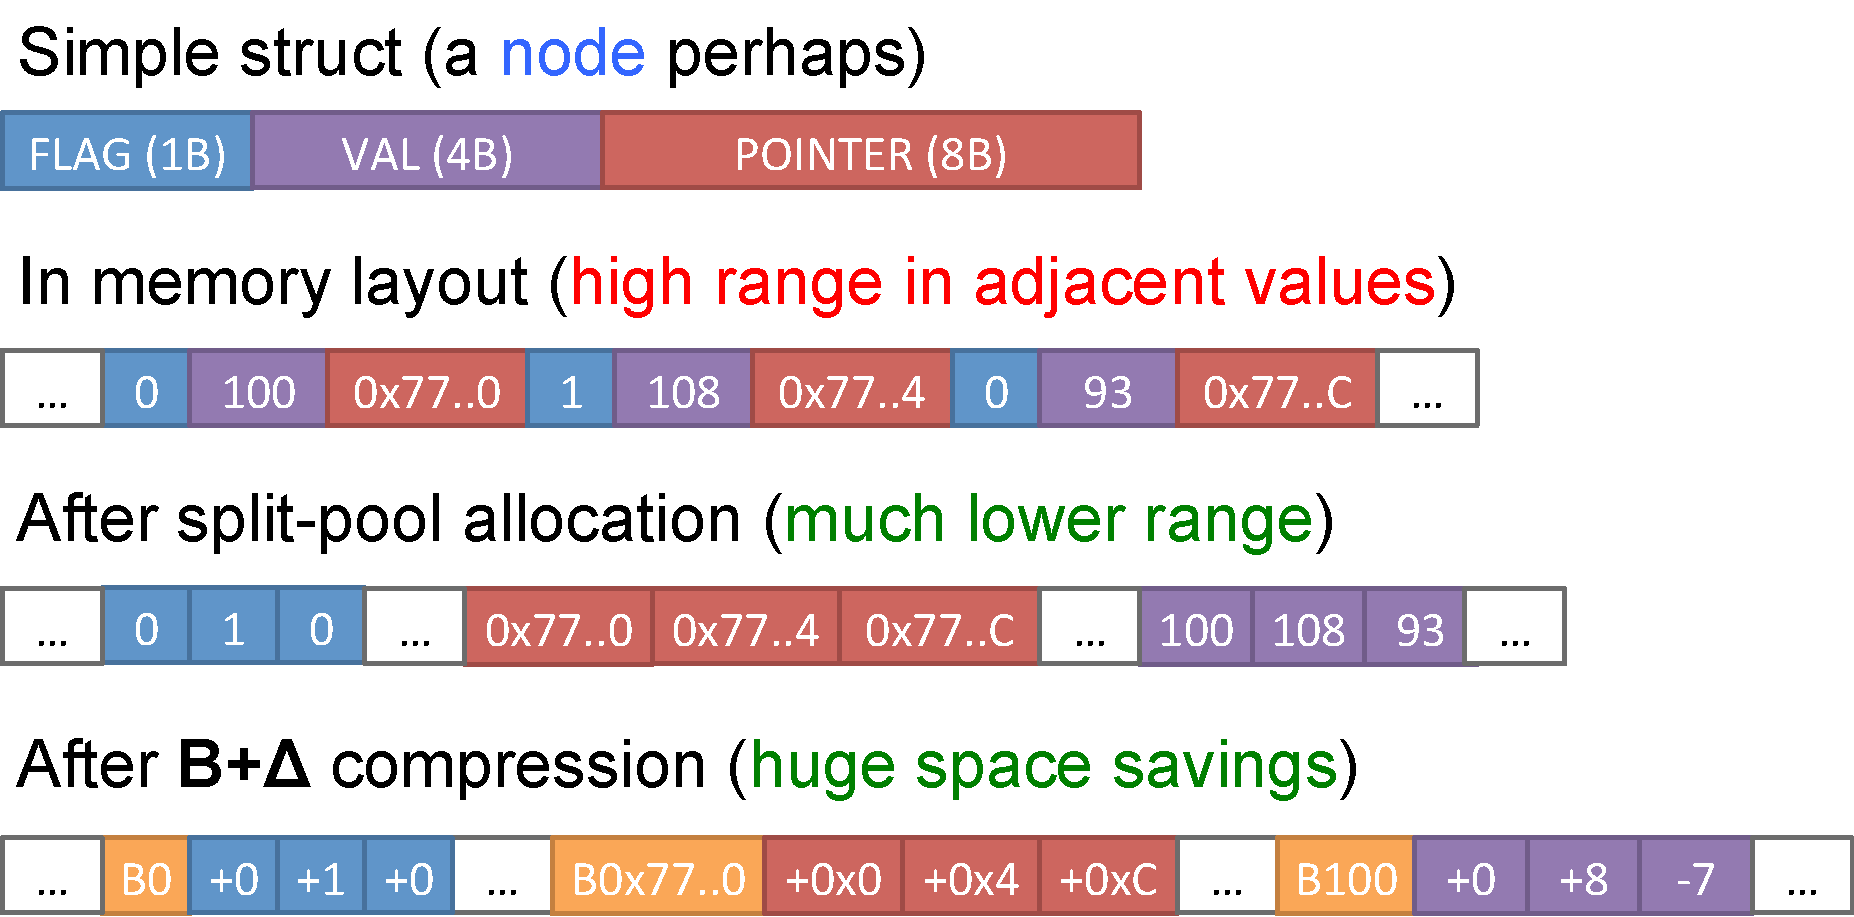
\includegraphics[scale=0.27]{mechanisms.pdf}
\end{figure}

\subsection{Caveats}
Some simplifications were made to the above examples for that sake of brevity. For example, a long string of boolean flags in memory is seldom B+$\Delta$-compressible. This is because B+$\Delta$ compression operates at 4-byte and 8-byte granularities. A string of 32 or 64 booleans has high entropy, even for biased distributions for true and false values. Interpreting these strings as integers and computing the differences may result in very large deltas, and low compressibility.


\section{Evaluation Methodology}
This paper intends to show proof of concept. As such, we opted to evaluate over more specific metrics than straight IPC performance. Instead, we are more interested in compression ratio and a subsequent increase in hit rate. We expect these metrics to strongly correlate with the computed IPC on a cycle accurate simulator.

We measure compression ratio for a given benchmark as follows, where $util$ is the amount of cache space in use. The higher the better.
\[
CompressionRatio = \frac{Util_{\text{baseline}}}{Util_{\text{implementation}}}
\]

\subsection{Benchmark Selection}
Only three benchmarks were used in this study. This is largely because we have yet to implement the pointer transformations necessary for splitting and pooling in the LLVM compiler. Thus, programs had to be converted manually, were smaller in size, and have smaller working sets. We refer to these programs as micro-benchmarks.

Because of our limited benchmark suite, the programs were chosen carefully. We were particularly interested in how splitting and pooling might expose \textit{value}-locality in memory, even in pointer heavy algorithms with objects. A brief description of our micro-benchmarks follows:

\begin{itemize}
\item{\textbf{LLU:} Linked list traversal. Lists are grown each iteration, and counters within each node are incremented. This is an approximation for the better known\textit{Health} micro-benchmark.}
\item{\textbf{Bisort:} This performs a bitonic sort on a randomly generated tree.}
\item{\textbf{ArraySort:} A simple array sort. Elements are swapped and copied by value, not by pointer.}
\end{itemize}


\subsection{Manual Splitting and Pooling}
Splitting objects and pooling their members appropriately was done manually. Later we intend to perform these transformations in the compiler. Nevertheless, there are several drawbacks to this approach.

Firstly, hand optimized code-quality is not necessarily achievable by a compiler. As a programmer, one has perfect information about safety, problem size, and the type of data intended for each struct member. Second, pooling often incurs a static memory overhead\cite{mpads}  because the last pool is not always filled (but memory is still reserved).

We acknowledge that these factors concede some fidelity from the results. However, because this study is a proof of concept, we felt this was appropriate compromise.


\subsection{Cache Simulators}
Only a single level memory hierarchy is simulated here. Even though B+$\Delta$ compression is intended to run below the L1 cache, we do not omit L1 hits from our data. Normally the L2 would never see these requests. However, the validity of the data holds as both the baseline and B+$\Delta$ caches appreciate a proportional increase in hits.

\textbf{Baseline simulator} -- a 16-way, 32-byte block cache. The cache size is varied throughout the study to observe the interaction between capacity, the working set of the program, and the hit rate. The baseline cache implements a perfect least recently used (LRU) policy.

\textbf{B+$\Delta$ cache simulator} -- a 16-way, 32-byte block cache. This cache performs B+$\Delta$ style compression on inserted cache lines. Again, the cache capacity is varied throughout the study to observe the effect of small space constraints, large working sets, and pooling.

The simulator implements a perfect LRU policy. When a newly inserted cache line exceeds the size of the set, LRU blocks are evicted until the new block fits. Recent literature, such as Cache Aware Replacement Policies\cite{carp} (CARP) suggests many optimizations to this policy, but they are not simulated here.

\begin{figure}[bp]
  \centering
    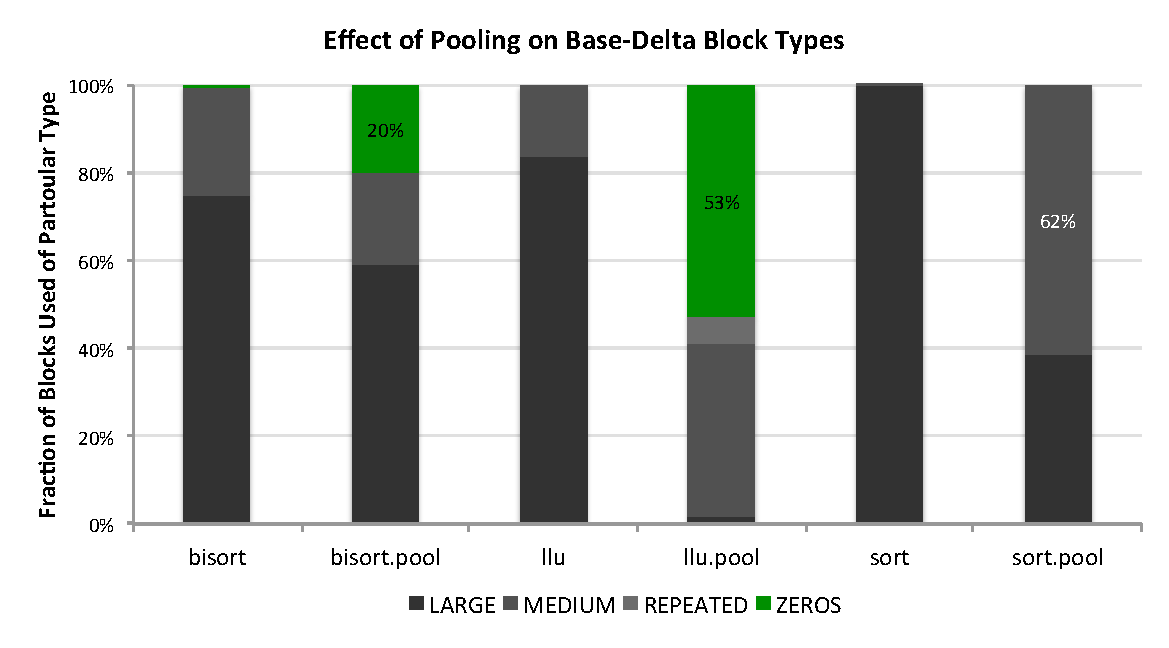
\includegraphics[width=\linewidth]{pooling-effect.pdf}
  \caption{Effect of splitting and pooling on B+$\Delta$ compression.}
\end{figure}

\section{Results and Analysis}

\subsection{Effects of Splitting and Pooling on Block Types}
For a sanity check, we first look at the block types that occur in a B+$\Delta$ compressed cache with splitting and pooling, and without. Figure 2 shows each benchmark paired with its split-pool transformed counterpart.

Without splitting and pooling, B+$\Delta$ compression is able to effectively compress about 20\% of the total number of blocks allocated (with the exception of the \textit{sort} micro-benchmark). By effective, we mean that a compression ratio of 1.5 or greater is achieved. These are labeled as \textit{medium} blocks. \textit{Large} blocks are either incompressible (represented with the full 32 bytes) or obtain very little space savings.

With splitting and pooling, however, we observe a substantial increase in blocks that are \textit{zero}, \textit{repeated}, and \textit{medium} compressible. The increase in \textit{zero}-type blocks is particularly promising, because they can be encoded with only 1 byte using B+$\Delta$. \textbf{Overall, we improve the ratio of effectively compressed blocks from 20\% to 68\%.} This is an excellent result. 


\subsection{Varying the Cache Size}
As the cache size is increased, we see a very different trend past the 64KB mark. This is because the average working memory set of our micro-benchmark suite is about 90KB. When a program's working set is larger than the cache capacity, we incur a much greater fraction of conflict and capacity misses. Under these conditions, the cache stays full once it has warmed up, and behaves differently thusly. We elaborate on the dichotomy between the left and right sides of figures 3 and 4 below.


\subsection{Effect on Compression Ratio}
Figure 3 shows the compression ratio each implementation achieves with respect to the baseline cache. On the left of Figure 3, we observe that the baseline, pooling, and B+$\Delta$ implementation achieve no \textit{relative} compression because they all fill the cache to capacity while trying and accommodate the working set. 

B+$\Delta$ with splitting and pooling performs substantially better than all other implementations. We attribute the improvement over standalone B+$\Delta$ compression to the better \textit{value}-locality exposed by pooling. For cases where the cache capacity is smaller than the working set, we achieve a worst case 20\% improvement over the baseline.

On the right of figure 3, cache capacities are greater than the working set. We see little variation between a particular implementation across cache size. This is because they are all able to accommodate the memory needs of the programs. B+$\Delta$ with splitting and pooling \textbf{outperforms the other configurations by about 2.8X}. As an aside, we observe relatively how much more space it takes for the other implementations to encode the working set in the cache.

A quick glance at the right side of Figure 4 indicates that we do not realize performance gains over the baseline for hit-rate, despite achieving large space savings. We explain this below. We believe these space saving will become increasingly important in multiprogrammed environments, as they could mitigate cache pollution and memory interference.

\subsection{Effect on Hit Rate}

Figure 4 shows the hit rate each implementation achieves with respect to the baseline. A brief inspection illuminates the same dichotomy in behavior around the size of the working set. We will explain each side in detail. 

On the left of Figure 4, the working set of the micro-benchmark programs is larger than the cache capacity. Keeping useful data in the cache is strained by capacity and conflict misses, which lead to evictions. Compression benefits manifest themselves very clearly under such conditions. Encoding more data in the cache effectively increases the capacity (both overall and in each set), and mitigates the high miss-and-evict rate.

As in prior work B+$\Delta$ offers some performance gains here. Standalone splitting and pooling does as well. We attribute this to the fact that such techniques improve locality in general.

B+$\Delta$ with splitting and pooling again outperforms considerably by about \textbf{12\% over the baseline}. As the cache capacity approaches the size of the working memory set, the gains become less substantial. This is because the other configurations become less constrained for space.

On the right side of Figure 4, the cache capacities are larger than working set. Because all configurations can handle the data footprint, we see no relative gains of on over another. Performance distinctions become much clearer as you place the system under more pressure.

\begin{figure}
  \centering
    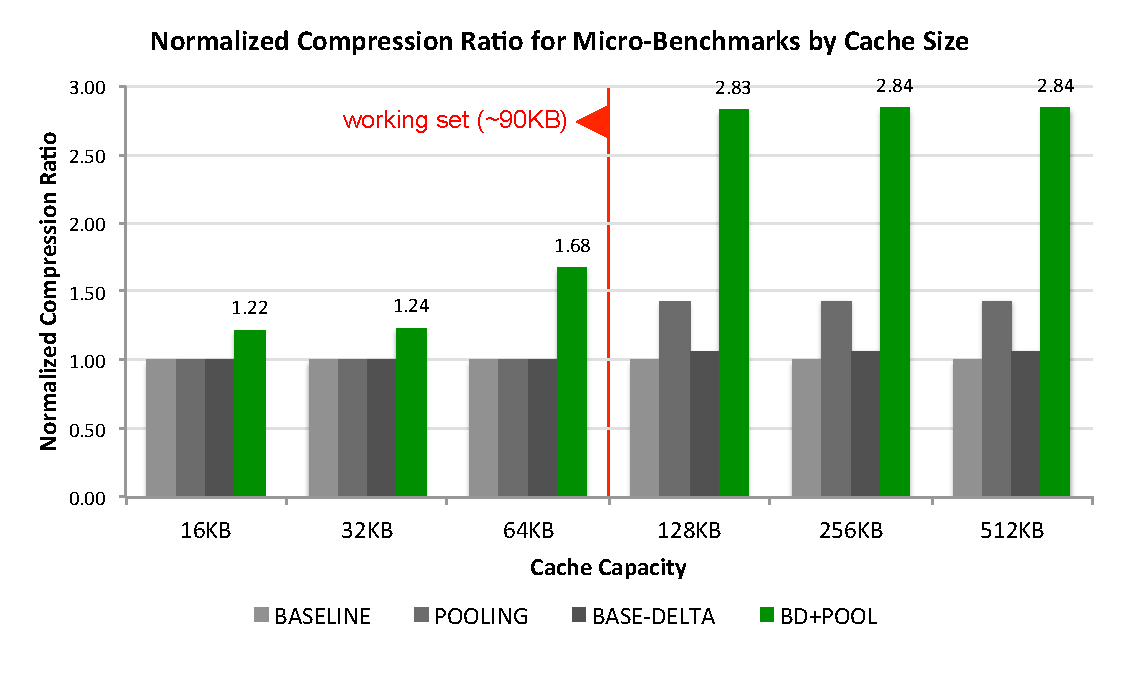
\includegraphics[width=\linewidth]{size2compression.pdf}
  \caption{Average normalized compression ratio for various cache sizes.}
\end{figure}

\begin{figure}
  \centering
    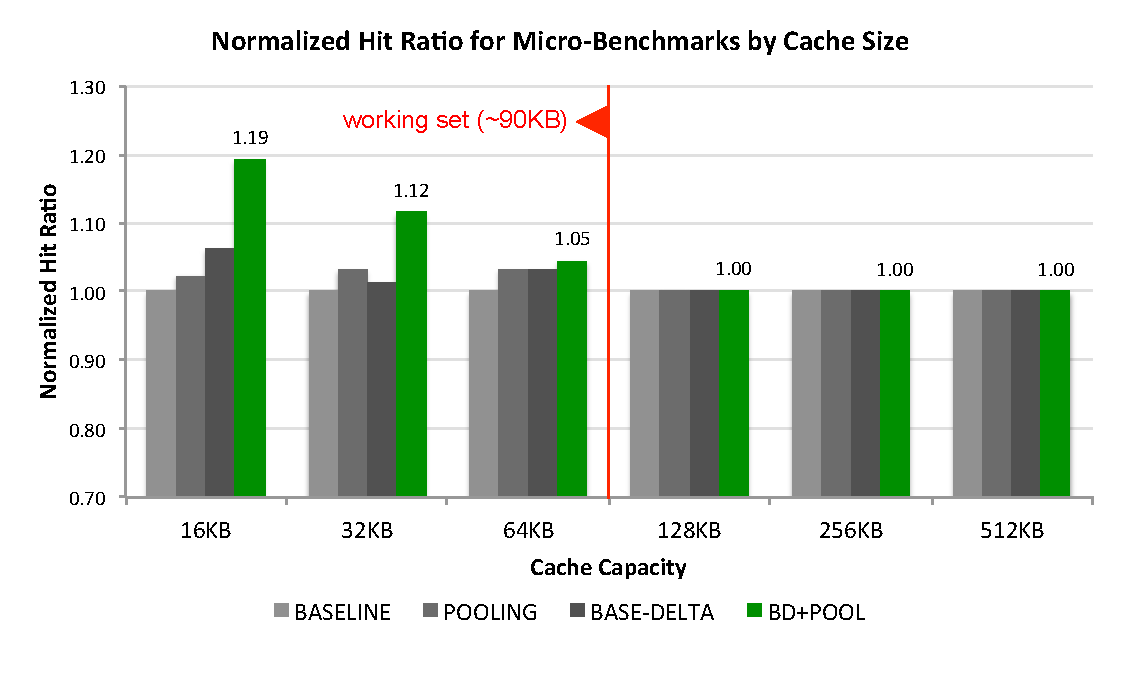
\includegraphics[width=\linewidth]{size2hits.pdf}
  \caption{Average normalized hit ratio for various cache sizes.}
\end{figure}


\section{Conclusions}
This paper presents a strong case for further exploration of using B+$\Delta$ compression techniques in tandem with data splitting and memory pooling. We describe how using splitting and pooling principles we can expose large, contiguous regions of memory with high \textit{value}-locality. That is, stretches with low dynamic range that B+$\Delta$ compression can leverage with higher probability.

We show experimentally that programs restructured in this manner yield smaller block types within B+$\Delta$ encoding, and substantially high compression ratios over the baseline cache with no B+$\Delta$ compression or memory pooling and splitting.

 Next, we discuss the shape of the data, identifying the dichotomy in cache behavior when the working memory set is large or smaller than the cache capacity. In general, the advantages of B+$\Delta$ with splitting and pooling become more apparent as the cache space constricts.

Finally, an aggregation of the results shows that B+$\Delta$ with splitting and pooling outperforms each other configuration alone, including the baseline. We observe an average compression ratio of about 2.8X over the baseline while holding the entire working set in the cache. Lastly, we see a 12\% average improvement in hit-rate over the baseline under constrained cache space conditions.


\section{Further Work}
This work has a number shortcomings. First our (micro) benchmarks are small and the data transformations were done by hand. To obtain higher fidelity data, we will need to transform larger more standard benchmarks. For feasibility reasons, this cannot be done manually.

Therefore, the next steps involve implementing these pointer transformations in the LLVM compiler--LLVM is open source. There is a good body of work on how to approach this problem\cite{mpads}. These larger programs will prove more representative of the workloads a real system would place on our modified B+$\Delta$ compression idea.

Second, this study does not directly measure performance. To do so, we will need to run our \textit{transformed} benchmarks on a cycle accurate simulator that implements B+$\Delta$ compression. From here, we can obtain data on absolute performance gains.

After these steps, we can better gauge how the various overheads of automated splitting and pooling will affect performance. Recall the static memory footprint pooling incurs for underutilized pools. In addition there are various other inefficiencies such as value padding, among other things.

Finally, it would be great to see how B+$\Delta$ compression with splitting and pooling interacts with non-vanilla LRU replacement policies. As mentioned, there this area has already received some attention\cite{carp}. I suspect the ideas in this paper could benefit greatly from these studies.


\bstctlcite{bstctl:etal, bstctl:nodash, bstctl:simpurl}
\bibliographystyle{IEEEtranS}
\bibliography{references}

\end{document}

